\documentclass{../ucll-slides}
\usepackage{pxfonts}
\usepackage{tikz}
\usepackage{calc}
\usepackage{../ucll-code}


\usetikzlibrary{calc,shadows,tikzmark}

\coursename{Distributed Applications}
\title{Processes}


\begin{document}

\maketitle

\section{OS Refresher}

\begin{frame}
    \frametitle{Operating Systems Refresher}
    \begin{center}
        \begin{tikzpicture}[os/.style={draw,drop shadow,fill=blue!50},
                            process/.style={draw,drop shadow,fill=red!50},
                            process header/.style={font=\sc\bf\Large,red,opacity=0.5},
                            hardware/.style={drop shadow,fill=magenta!50},
                            cpu/.style={draw,minimum width=1cm,minimum height=1cm,drop shadow,fill=magenta!75},
                            note/.style={drop shadow,fill=green!50,inner sep=5mm},
                            note arrow/.style={-latex,ultra thick}]
            \node[os,minimum width=10cm,minimum height=1cm] (os) {Operating System};
            \coordinate (process a) at ($ (os.south west) + (0,-0.2) $);
            \coordinate (process b) at ($ (os.south west) ! 0.35 ! (os.south east) + (0,-0.2) $);
            \coordinate (process c) at ($ (os.south west) ! 0.7 ! (os.south east) + (0,-0.2) $);
            \draw[process] (process a) rectangle ++(3,-4);
            \draw[process] (process b) rectangle ++(3,-4);
            \draw[process] (process c) rectangle ++(3,-4);
            \node[anchor=north west,minimum width=3cm,process header] at (process a) {Process A};
            \node[anchor=north west,minimum width=3cm,process header] at (process b) {Process B};
            \node[anchor=north west,minimum width=3cm,process header] at (process c) {Process C};

            \begin{scope}[xshift=-4cm,yshift=-4cm]
                \coordinate (thread 1 start) at (0,0);
                \coordinate (thread 1 end) at (0,1);
                \draw[smooth,thick] plot[tension=1] coordinates{(0,0) (1,1) (0,2) (0,1)};
            \end{scope}

            \begin{scope}[xshift=-1cm,yshift=-4cm]
                \coordinate (thread 2 start) at (0,0);
                \coordinate (thread 2 end) at (0,1);
                \coordinate (thread 3 start) at (2,0);
                \coordinate (thread 3 end) at (1.8,0.5);
                \draw[smooth,thick] plot[tension=1] coordinates{(0,0) (1,2) (1,1) (0,1)};
                \draw[smooth,thick] plot[tension=1] coordinates{(2,0) (2,2) (1.5,1) (1.8,0.5)};
            \end{scope}

            \begin{scope}[xshift=2.5cm,yshift=-4cm]
                \coordinate (thread 4 start) at (0,2);
                \coordinate (thread 4 end) at (1,0.5);
                \coordinate (thread 5 start) at (2,0);
                \coordinate (thread 5 end) at (1.8,0.5);
                \coordinate (thread 6 start) at (0,0);
                \coordinate (thread 6 end) at (1.7,0.25);
                \draw[smooth,thick] plot[tension=1] coordinates{(1,1) (0,2) (0,1) (0.5,0) (1,0.5)};
                \draw[smooth,thick] plot[tension=1] coordinates{(2,0) (2,2) (1.5,1) (1.8,0.5)};
                \draw[smooth,thick] plot[tension=1] coordinates{(0,0) (1,2) (0.5,1.5) (1.7,0.25)};
            \end{scope}

            \begin{scope}[xshift=-5cm,yshift=-7cm]
                \draw[hardware] (0,0) rectangle ++(10,2);
                \node[cpu,anchor=south west] (cpu 1) at (1.5,0.5) {core};
                \node[cpu,anchor=south west] (cpu 2) at (3.5,0.5) {core};
                \node[cpu,anchor=south west] (cpu 3) at (5.5,0.5) {core};
                \node[cpu,anchor=south west] (cpu 4) at (7.5,0.5) {core};
            \end{scope}

            \only<2>{
                \node[note,anchor=south] (note) at ($ (process b) + (0,1) $) { Processes };
                \draw[note arrow] (note) -- (process a);
                \draw[note arrow] (note) -- (process b);
                \draw[note arrow] (note) -- (process c);
            }

            \only<3>{
                \node[note,anchor=south west] (note) at ($ (process a) + (1,1) $) {
                    \parbox{6cm}{
                        Each process lives in its own virtual memory space.
                        Processes can't peek in each other's memory spaces.
                    }
                };
                \draw[ultra thick,black,fill=black] ($ (process b) + (-0.3,0) $) rectangle ++(0.1,-4);
                \draw[ultra thick,black,fill=black] ($ (process c) + (-0.3,0) $) rectangle ++(0.1,-4);
            }

            \only<4>{
                \node[note,anchor=south west] (note) at ($ (process a) + (1,1) $) {
                    Threads.
                };
                \draw[note arrow] (note) -- (thread 1 end);
                \draw[note arrow] (note) -- (thread 2 end);
                \draw[note arrow] (note) -- (thread 3 end);
                \draw[note arrow] (note) -- (thread 4 start);
                \draw[note arrow] (note) -- (thread 5 end);
                \draw[note arrow] (note) -- (thread 6 start);
            }

            \only<5>{
                \node[note] (note) at (0,-2.5) {
                    \parbox{6cm}{
                        Threads are sequences of instructions that run in parallel
                        (or so we say, see later).
                    }
                };
            }

            \only<6>{
                \node[note] (note) at (0,-2.5) {
                    \parbox{6cm}{
                        Threads in the same process share memory space.
                        What one thread does, the other ones can see.
                    }
                };
            }

            \only<7>{
                \node[note,anchor=south west] (note) at ($ (process a) + (1,1) $) {
                    Each thread needs a CPU core to run on.
                };
                \draw[note arrow] (thread 1 start) -- (cpu 1);
                \draw[note arrow] (thread 2 start) -- (cpu 2);
                \draw[note arrow] (thread 3 start) -- (cpu 3);
                \draw[note arrow] (thread 4 end) -- (cpu 4);
            }

            \only<8>{
                \node[note] (note) at (0,-2.5) {
                    \parbox{6cm}{
                        Often there are thousands of threads, but only a couple of cores (2--32 as of 2019).
                        It is therefore impossible to assign a core to each thread.
                    }
                };
            }

            \only<9>{
                \node[note] (note) at (0,-2.5) {
                    \parbox{6cm}{
                        Solution: each thread gets to run for a limited time (milliseconds) on a core,
                        and is then interrupted (pre-emptive multithreading) to make room for another thread.
                    }
                };
            }
        \end{tikzpicture}
    \end{center}
\end{frame}

\end{document}

%%% Local Variables:
%%% mode: latex
%%% TeX-master: t
%%% End:
